\section{System's Perspective}


% \textcolor{red}{Design and architecture of your ITU-MiniTwit systems.}

Our ITU-MiniTwit system consists of a web service and an API service which act in a client-server architecture deployed in a Docker Swarm on virtual machines on Digital Ocean. 
The system is load balanced using Nginx. Data is stored in a PostgreSQL database that is deployed on Digital Ocean. 
The UML deployment diagram in figure \ref{fig:deployment} shows how the different components in our system are deployed.

\begin{figure}[h]
    \centering
    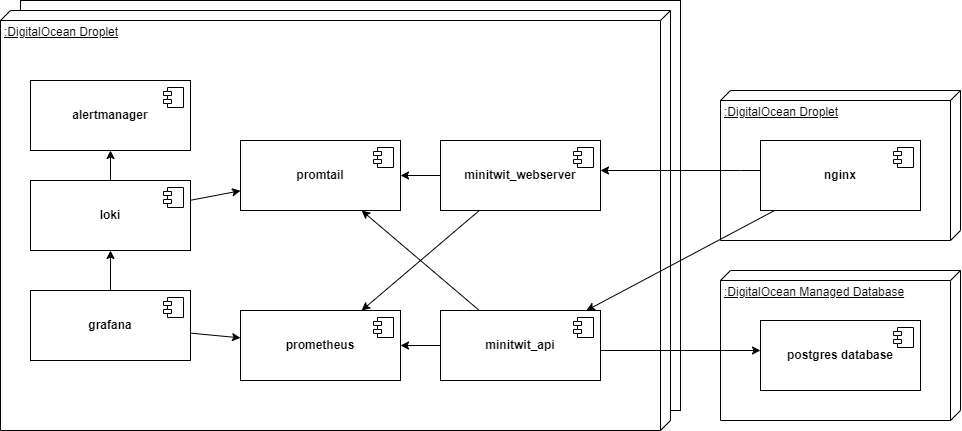
\includegraphics[width=0.9\textwidth]{images/deployment.png}
    \caption{UML Deployment Diagram}
    \label{fig:deployment}
\end{figure}

The web service and API service are both written in Golang, using Go/Gorilla for routing and session management. Initially we had decided to write it in Crystal/Kemal, but we soon discovered that Kemal's documentation was insufficient, making it challenging to work with. Consequently, we switched to Golang, which offered similar features but had much more comprehensive documentation. 
A detailed feature mapping of the system and a comparison of programming languages can be found in Appendix \ref{app:programming_language_choice}. 

%\textcolor{red}{ All dependencies of your ITU-MiniTwit systems on all levels of abstraction and development stages. That is, list and briefly describe all technologies and tools you applied and depend on.}
For an overview and concise description of the technologies and tools utilized throughout our project work, see Appendix \ref{app:technologies_and_tools}. Each technology will also be introduced throughout the report.


%\subsubsection*{List of Technologies and Tools Utilized}

%\begin{multicols}{2}
%    \begin{itemize}
%        \item \textbf{Go}: A statically typed, compiled programming.
%        \item \textbf{Go/Gorilla}: Used for routing and session management.
%        \item \textbf{SQLite}: Used initially and for testing.
%        \item \textbf{Docker}: Containerization is used deliberately throughout our system and in delivery.
%        \item \textbf{Docker Swarm}: Container orchestration tool.
%        \item \textbf{DigitalOcean}: Used for virtualization and managed database.
%        \item \textbf{Prometheus}: Used for monitoring metrics.
%        \item \textbf{Grafana}: Used to visualize our data and metrics.
%        \item \textbf{PostgreSQL}: Used after the transition from SQLite and managed by DigitalOcean.
%        \item \textbf{Promtail}: Used for gathering logs.
%        \item \textbf{Loki}: Used for log aggregation, with Grafana for log querying and visualization.
%        \item \textbf{Nginx}: Used for load balancing.
%        \item \textbf{CertBot}: Used for automatically using Let's Encrypt certificates to enable HTTPS on web servers.
%        %\item \textbf{Terraform}: An infrastrcucture as code tool that allows users to define and provision data center infrastructure using a high-level configuration language. 
%    \end{itemize}
%\end{multicols}
%\textcolor{red}{Shorten s.t. we specify what it is used for instead of the generic 'what is it'}

% \subsubsection*{Technology choices}%should maybe just be in text when relevant

% \red{MSc should argue for the choice of technologies and decisions for at least all cases for which we asked you to do so in the tasks at the end of each session.}

\subsection{Subsystem interactions}

% \red{Important interactions of subsystems.
% For example, via an illustrative UML Sequence diagram that shows the flow of information through your system from user request in the browser, over all subsystems, hitting the database, and a response that is returned to the user.
% Similarly, another illustrative sequence diagram that shows how requests from the simulator traverse your system.}

The interactions that a user accessing our web client and the interactions the simulator undergo are similar. 
Figure \ref{fig:user_sequence} is a sequence diagram depicting the order of operations when a user visits the web client and hits the public timeline -- from Nginx to the database and back again. 
Similarly, figure \ref{fig:sim_sequence} is a sequence diagram depicting the order of operations when the simulator sends a request to post a message for a given user.

% Figure \ref{fig:user_sequence} shows the flow of information seen from the perspective of a user accessing the website. Initially the user reaches the load balancer, nginx, connecting and forwarding the request to one of the webserver replicas that then looks back to nginx with a request for a backend api. When the backend receives the request it sends the query for recent messages to the database as well as logs and updates monitoring metrics before returning the response to nginx and then to the webserver. Ultimately the webserver serves the final page to the user through nginx using the messages received from the backend.


\begin{figure}[H]
    \centering
    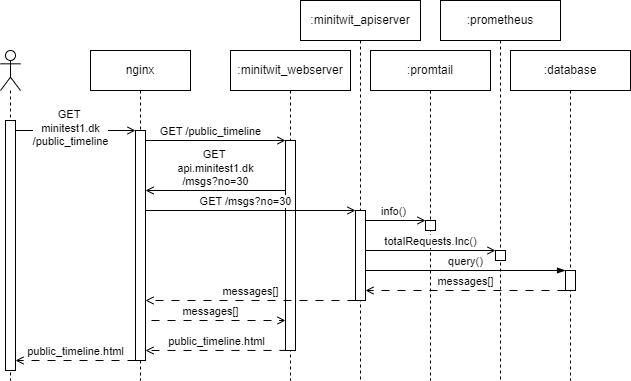
\includegraphics[width=0.8\textwidth]{images/sequence.png}
    \caption{Sequence diagram of the user interacting with the system.}
    \label{fig:user_sequence}
\end{figure}

% The simulator interaction is very similar to the interaction of the user except for the fact that it does not need to go through the webserver. The flow of a POST request can be seen in the sequence diagram in figure \ref{fig:sim_sequence}. 
One thing to note is that we have not been stress testing the user perspective in this course as all requests have come from the simulator. This means that we do not have data to reflect on the performance of our nginx setup which results in a lot of back and forth messaging as seen in the first diagram. 

\begin{figure}[H]
    \centering
    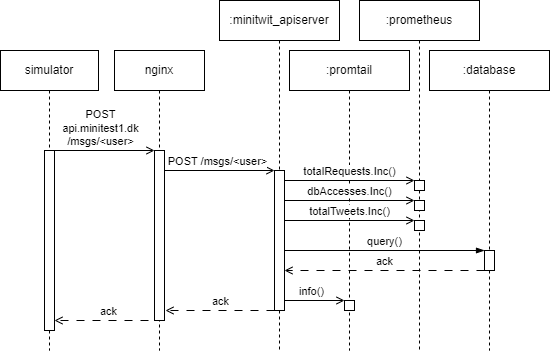
\includegraphics[width=0.8\textwidth]{images/sequence-simulator.png}
    \caption{Sequence diagram of the simulator interacting with the system.}
    \label{fig:sim_sequence}
\end{figure}




\subsection{Current state}
\label{sec:current-state}
%\textcolor{red}{Describe the current state of your systems, for example using results of static analysis and quality assessments.}

At the time of writing, our ITU-MiniTwit system is being evaluated using the static code analysis tools, Code Climate and SonarCloud.
For an overview, see Appendix \ref{app:static_analysis}. In summary, both tools reveal that while the system has a good level of maintainability and security, the following areas require improvement:

\begin{itemize}
    \item \textbf{Code Smells}: Identified in Code Climate, these primarily consist of functions with an excessive length and functions with multiple return statements. 
    \item \textbf{Duplications}: Identified in SonarCloud, we exceed the suggested amount of duplicated code. This is primarily duplicated code blocks between our API and the front-end, related to database connections.  
    \item \textbf{Test Coverage}: Implementing and configuring comprehensive test coverage to accurately reflect this metric in both Code Climate and SonarCloud.
    \item \textbf{Maintainability issues}: The specific issues noted in SonarCloud should be resolved according to their estimated effort to maintain and ensure a low technical debt ratio.
\end{itemize}

Addressing these areas will improve the current state of our codebase and ensure long-term maintainability. During the project we have listened to the feedback from these tools and made changes. 
In one instance we refactored our api and src directories from being a single python file to many different files based on their responsibilities resulting in an easier overview of the code base and increasing maintainability.
